\documentclass[twoside]{book}

% Packages required by doxygen
\usepackage{fixltx2e}
\usepackage{calc}
\usepackage{doxygen}
\usepackage[export]{adjustbox} % also loads graphicx
\usepackage{graphicx}
\usepackage[utf8]{inputenc}
\usepackage{makeidx}
\usepackage{multicol}
\usepackage{multirow}
\PassOptionsToPackage{warn}{textcomp}
\usepackage{textcomp}
\usepackage[nointegrals]{wasysym}
\usepackage[table]{xcolor}

% Font selection
\usepackage[T1]{fontenc}
\usepackage[scaled=.90]{helvet}
\usepackage{courier}
\usepackage{amssymb}
\usepackage{sectsty}
\renewcommand{\familydefault}{\sfdefault}
\allsectionsfont{%
  \fontseries{bc}\selectfont%
  \color{darkgray}%
}
\renewcommand{\DoxyLabelFont}{%
  \fontseries{bc}\selectfont%
  \color{darkgray}%
}
\newcommand{\+}{\discretionary{\mbox{\scriptsize$\hookleftarrow$}}{}{}}

% Page & text layout
\usepackage{geometry}
\geometry{%
  a4paper,%
  top=2.5cm,%
  bottom=2.5cm,%
  left=2.5cm,%
  right=2.5cm%
}
\tolerance=750
\hfuzz=15pt
\hbadness=750
\setlength{\emergencystretch}{15pt}
\setlength{\parindent}{0cm}
\setlength{\parskip}{3ex plus 2ex minus 2ex}
\makeatletter
\renewcommand{\paragraph}{%
  \@startsection{paragraph}{4}{0ex}{-1.0ex}{1.0ex}{%
    \normalfont\normalsize\bfseries\SS@parafont%
  }%
}
\renewcommand{\subparagraph}{%
  \@startsection{subparagraph}{5}{0ex}{-1.0ex}{1.0ex}{%
    \normalfont\normalsize\bfseries\SS@subparafont%
  }%
}
\makeatother

% Headers & footers
\usepackage{fancyhdr}
\pagestyle{fancyplain}
\fancyhead[LE]{\fancyplain{}{\bfseries\thepage}}
\fancyhead[CE]{\fancyplain{}{}}
\fancyhead[RE]{\fancyplain{}{\bfseries\leftmark}}
\fancyhead[LO]{\fancyplain{}{\bfseries\rightmark}}
\fancyhead[CO]{\fancyplain{}{}}
\fancyhead[RO]{\fancyplain{}{\bfseries\thepage}}
\fancyfoot[LE]{\fancyplain{}{}}
\fancyfoot[CE]{\fancyplain{}{}}
\fancyfoot[RE]{\fancyplain{}{\bfseries\scriptsize Generated by Doxygen }}
\fancyfoot[LO]{\fancyplain{}{\bfseries\scriptsize Generated by Doxygen }}
\fancyfoot[CO]{\fancyplain{}{}}
\fancyfoot[RO]{\fancyplain{}{}}
\renewcommand{\footrulewidth}{0.4pt}
\renewcommand{\chaptermark}[1]{%
  \markboth{#1}{}%
}
\renewcommand{\sectionmark}[1]{%
  \markright{\thesection\ #1}%
}

% Indices & bibliography
\usepackage{natbib}
\usepackage[titles]{tocloft}
\setcounter{tocdepth}{3}
\setcounter{secnumdepth}{5}
\makeindex

% Hyperlinks (required, but should be loaded last)
\usepackage{ifpdf}
\ifpdf
  \usepackage[pdftex,pagebackref=true]{hyperref}
\else
  \usepackage[ps2pdf,pagebackref=true]{hyperref}
\fi
\hypersetup{%
  colorlinks=true,%
  linkcolor=blue,%
  citecolor=blue,%
  unicode%
}

% Custom commands
\newcommand{\clearemptydoublepage}{%
  \newpage{\pagestyle{empty}\cleardoublepage}%
}

\usepackage{caption}
\captionsetup{labelsep=space,justification=centering,font={bf},singlelinecheck=off,skip=4pt,position=top}

%===== C O N T E N T S =====

\begin{document}

% Titlepage & ToC
\hypersetup{pageanchor=false,
             bookmarksnumbered=true,
             pdfencoding=unicode
            }
\pagenumbering{alph}
\begin{titlepage}
\vspace*{7cm}
\begin{center}%
{\Large e\+Jkiva }\\
\vspace*{1cm}
{\large Generated by Doxygen 1.8.14}\\
\end{center}
\end{titlepage}
\clearemptydoublepage
\pagenumbering{roman}
\tableofcontents
\clearemptydoublepage
\pagenumbering{arabic}
\hypersetup{pageanchor=true}

%--- Begin generated contents ---
\chapter{Hierarchical Index}
\section{Class Hierarchy}
This inheritance list is sorted roughly, but not completely, alphabetically\+:\begin{DoxyCompactList}
\item \contentsline{section}{controller.\+Customer\+Controller}{\pageref{classcontroller_1_1_customer_controller}}{}
\item \contentsline{section}{repository.\+Customer\+Repository}{\pageref{classrepository_1_1_customer_repository}}{}
\item \contentsline{section}{customer.\+Customer\+Test}{\pageref{classcustomer_1_1_customer_test}}{}
\item \contentsline{section}{utils.\+Hibernate\+Utils}{\pageref{classutils_1_1_hibernate_utils}}{}
\item \contentsline{section}{controller.\+Login\+Controller}{\pageref{classcontroller_1_1_login_controller}}{}
\item \contentsline{section}{controller.\+Manager\+Controller}{\pageref{classcontroller_1_1_manager_controller}}{}
\item \contentsline{section}{repository.\+Manager\+Repository}{\pageref{classrepository_1_1_manager_repository}}{}
\item \contentsline{section}{controller.\+Operator\+Controller}{\pageref{classcontroller_1_1_operator_controller}}{}
\item \contentsline{section}{repository.\+Operator\+Repository}{\pageref{classrepository_1_1_operator_repository}}{}
\item Serializable\begin{DoxyCompactList}
\item \contentsline{section}{entity.\+Authomach}{\pageref{classentity_1_1_authomach}}{}
\item \contentsline{section}{entity.\+Carries}{\pageref{classentity_1_1_carries}}{}
\item \contentsline{section}{entity.\+Carries\+Id}{\pageref{classentity_1_1_carries_id}}{}
\item \contentsline{section}{entity.\+Departament}{\pageref{classentity_1_1_departament}}{}
\item \contentsline{section}{entity.\+Order}{\pageref{classentity_1_1_order}}{}
\item \contentsline{section}{entity.\+Orderproduct}{\pageref{classentity_1_1_orderproduct}}{}
\item \contentsline{section}{entity.\+Product}{\pageref{classentity_1_1_product}}{}
\item \contentsline{section}{entity.\+User}{\pageref{classentity_1_1_user}}{}
\item \contentsline{section}{entity.\+Usertype}{\pageref{classentity_1_1_usertype}}{}
\item \contentsline{section}{entity.\+Workstation}{\pageref{classentity_1_1_workstation}}{}
\end{DoxyCompactList}
\item \contentsline{section}{repository.\+User\+Repository}{\pageref{classrepository_1_1_user_repository}}{}
\end{DoxyCompactList}

\chapter{Class Index}
\section{Class List}
Here are the classes, structs, unions and interfaces with brief descriptions\+:\begin{DoxyCompactList}
\item\contentsline{section}{\mbox{\hyperlink{classentity_1_1_authomach}{entity.\+Authomach}} }{\pageref{classentity_1_1_authomach}}{}
\item\contentsline{section}{\mbox{\hyperlink{classentity_1_1_carries}{entity.\+Carries}} }{\pageref{classentity_1_1_carries}}{}
\item\contentsline{section}{\mbox{\hyperlink{classentity_1_1_carries_id}{entity.\+Carries\+Id}} }{\pageref{classentity_1_1_carries_id}}{}
\item\contentsline{section}{\mbox{\hyperlink{classcontroller_1_1_customer_controller}{controller.\+Customer\+Controller}} }{\pageref{classcontroller_1_1_customer_controller}}{}
\item\contentsline{section}{\mbox{\hyperlink{classentity_1_1_departament}{entity.\+Departament}} }{\pageref{classentity_1_1_departament}}{}
\item\contentsline{section}{\mbox{\hyperlink{classutils_1_1_hibernate_utils}{utils.\+Hibernate\+Utils}} }{\pageref{classutils_1_1_hibernate_utils}}{}
\item\contentsline{section}{\mbox{\hyperlink{classcontroller_1_1_login_controller}{controller.\+Login\+Controller}} }{\pageref{classcontroller_1_1_login_controller}}{}
\item\contentsline{section}{\mbox{\hyperlink{classentity_1_1_order}{entity.\+Order}} }{\pageref{classentity_1_1_order}}{}
\item\contentsline{section}{\mbox{\hyperlink{classentity_1_1_orderproduct}{entity.\+Orderproduct}} }{\pageref{classentity_1_1_orderproduct}}{}
\item\contentsline{section}{\mbox{\hyperlink{classentity_1_1_product}{entity.\+Product}} }{\pageref{classentity_1_1_product}}{}
\item\contentsline{section}{\mbox{\hyperlink{classentity_1_1_segment}{entity.\+Segment}} }{\pageref{classentity_1_1_segment}}{}
\item\contentsline{section}{\mbox{\hyperlink{classentity_1_1_user}{entity.\+User}} }{\pageref{classentity_1_1_user}}{}
\item\contentsline{section}{\mbox{\hyperlink{classentity_1_1_usertype}{entity.\+Usertype}} }{\pageref{classentity_1_1_usertype}}{}
\item\contentsline{section}{\mbox{\hyperlink{classentity_1_1_workstation}{entity.\+Workstation}} }{\pageref{classentity_1_1_workstation}}{}
\end{DoxyCompactList}

\chapter{Class Documentation}
\hypertarget{classentity_1_1_authomach}{}\section{entity.\+Authomach Class Reference}
\label{classentity_1_1_authomach}\index{entity.\+Authomach@{entity.\+Authomach}}


Inheritance diagram for entity.\+Authomach\+:\nopagebreak
\begin{figure}[H]
\begin{center}
\leavevmode
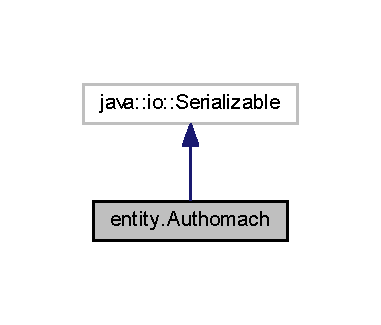
\includegraphics[width=183pt]{classentity_1_1_authomach__inherit__graph}
\end{center}
\end{figure}


Collaboration diagram for entity.\+Authomach\+:\nopagebreak
\begin{figure}[H]
\begin{center}
\leavevmode
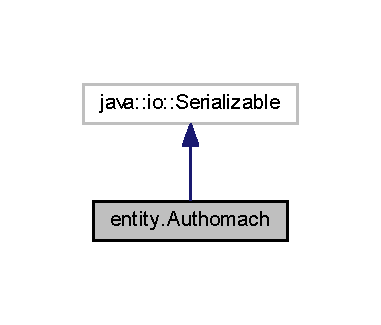
\includegraphics[width=183pt]{classentity_1_1_authomach__coll__graph}
\end{center}
\end{figure}
\subsection*{Public Member Functions}
\begin{DoxyCompactItemize}
\item 
\mbox{\Hypertarget{classentity_1_1_authomach_a8f9bf217f1a51601009ce0da96571cf2}\label{classentity_1_1_authomach_a8f9bf217f1a51601009ce0da96571cf2}} 
{\bfseries Authomach} (String description, Boolean state, Set carrieses)
\item 
\mbox{\Hypertarget{classentity_1_1_authomach_aa123815d3d8c471756c298edba10d4e1}\label{classentity_1_1_authomach_aa123815d3d8c471756c298edba10d4e1}} 
int {\bfseries get\+Machine\+Id} ()
\item 
\mbox{\Hypertarget{classentity_1_1_authomach_aa7eb52c9c1828f6870b84727cb2fd7d9}\label{classentity_1_1_authomach_aa7eb52c9c1828f6870b84727cb2fd7d9}} 
void {\bfseries set\+Machine\+Id} (int machine\+Id)
\item 
\mbox{\Hypertarget{classentity_1_1_authomach_ac935bc6cd52b576e53a3f58c6bb1eb1e}\label{classentity_1_1_authomach_ac935bc6cd52b576e53a3f58c6bb1eb1e}} 
String {\bfseries get\+Description} ()
\item 
\mbox{\Hypertarget{classentity_1_1_authomach_ab49dd6d37693e9b4a32e881aae5ec898}\label{classentity_1_1_authomach_ab49dd6d37693e9b4a32e881aae5ec898}} 
void {\bfseries set\+Description} (String description)
\item 
\mbox{\Hypertarget{classentity_1_1_authomach_a6c2b7c4d9aeb91c62791854f9f472b89}\label{classentity_1_1_authomach_a6c2b7c4d9aeb91c62791854f9f472b89}} 
Boolean {\bfseries get\+State} ()
\item 
\mbox{\Hypertarget{classentity_1_1_authomach_a7efa67cff55a9d3678745f918a26d7c8}\label{classentity_1_1_authomach_a7efa67cff55a9d3678745f918a26d7c8}} 
void {\bfseries set\+State} (Boolean state)
\end{DoxyCompactItemize}


\subsection{Detailed Description}
\mbox{\hyperlink{classentity_1_1_authomach}{Authomach}} generated by hbm2java 

The documentation for this class was generated from the following file\+:\begin{DoxyCompactItemize}
\item 
src/main/java/entity/Authomach.\+java\end{DoxyCompactItemize}

\hypertarget{classentity_1_1_carries}{}\section{entity.\+Carries Class Reference}
\label{classentity_1_1_carries}\index{entity.\+Carries@{entity.\+Carries}}


Inheritance diagram for entity.\+Carries\+:\nopagebreak
\begin{figure}[H]
\begin{center}
\leavevmode
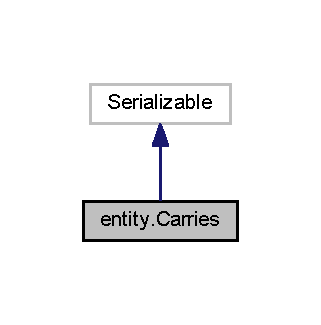
\includegraphics[width=154pt]{classentity_1_1_carries__inherit__graph}
\end{center}
\end{figure}


Collaboration diagram for entity.\+Carries\+:\nopagebreak
\begin{figure}[H]
\begin{center}
\leavevmode
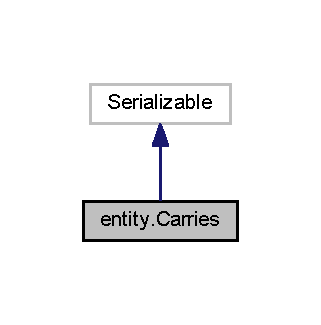
\includegraphics[width=154pt]{classentity_1_1_carries__coll__graph}
\end{center}
\end{figure}
\subsection*{Public Member Functions}
\begin{DoxyCompactItemize}
\item 
\mbox{\Hypertarget{classentity_1_1_carries_acf6db6a8bebc1383fb44b5d1a69db994}\label{classentity_1_1_carries_acf6db6a8bebc1383fb44b5d1a69db994}} 
{\bfseries Carries} (\mbox{\hyperlink{classentity_1_1_carries_id}{Carries\+Id}} id, \mbox{\hyperlink{classentity_1_1_orderproduct}{Orderproduct}} orderproduct)
\item 
\mbox{\Hypertarget{classentity_1_1_carries_a61138413c175da3c338dd6d3faf5034d}\label{classentity_1_1_carries_a61138413c175da3c338dd6d3faf5034d}} 
{\bfseries Carries} (\mbox{\hyperlink{classentity_1_1_carries_id}{Carries\+Id}} id, \mbox{\hyperlink{classentity_1_1_authomach}{Authomach}} authomach, \mbox{\hyperlink{classentity_1_1_orderproduct}{Orderproduct}} orderproduct, \mbox{\hyperlink{classentity_1_1_workstation}{Workstation}} workstation\+By\+Destiny\+Workstation\+Id, \mbox{\hyperlink{classentity_1_1_workstation}{Workstation}} workstation\+By\+Initial\+Workstation\+Id)
\item 
\mbox{\Hypertarget{classentity_1_1_carries_af1a678cc4d0ded3e9fecbf0a17a2ba3c}\label{classentity_1_1_carries_af1a678cc4d0ded3e9fecbf0a17a2ba3c}} 
\mbox{\hyperlink{classentity_1_1_carries_id}{Carries\+Id}} {\bfseries get\+Id} ()
\item 
\mbox{\Hypertarget{classentity_1_1_carries_a23d2ab3f05610f37bca03e7cc08ced73}\label{classentity_1_1_carries_a23d2ab3f05610f37bca03e7cc08ced73}} 
void {\bfseries set\+Id} (\mbox{\hyperlink{classentity_1_1_carries_id}{Carries\+Id}} id)
\item 
\mbox{\Hypertarget{classentity_1_1_carries_a539e6149274e7be94d86999d02af82d1}\label{classentity_1_1_carries_a539e6149274e7be94d86999d02af82d1}} 
\mbox{\hyperlink{classentity_1_1_authomach}{Authomach}} {\bfseries get\+Authomach} ()
\item 
\mbox{\Hypertarget{classentity_1_1_carries_a5fddad71e78d3206116e710916c8bb74}\label{classentity_1_1_carries_a5fddad71e78d3206116e710916c8bb74}} 
void {\bfseries set\+Authomach} (\mbox{\hyperlink{classentity_1_1_authomach}{Authomach}} authomach)
\item 
\mbox{\Hypertarget{classentity_1_1_carries_a6439c3d458849f3f5d87c0f9577fc16b}\label{classentity_1_1_carries_a6439c3d458849f3f5d87c0f9577fc16b}} 
\mbox{\hyperlink{classentity_1_1_orderproduct}{Orderproduct}} {\bfseries get\+Orderproduct} ()
\item 
\mbox{\Hypertarget{classentity_1_1_carries_af3856ed5dc8866063ed552e5a6289736}\label{classentity_1_1_carries_af3856ed5dc8866063ed552e5a6289736}} 
void {\bfseries set\+Orderproduct} (\mbox{\hyperlink{classentity_1_1_orderproduct}{Orderproduct}} orderproduct)
\item 
\mbox{\Hypertarget{classentity_1_1_carries_a13e9ee65fee8f33abd1b5fcd4da046c2}\label{classentity_1_1_carries_a13e9ee65fee8f33abd1b5fcd4da046c2}} 
\mbox{\hyperlink{classentity_1_1_workstation}{Workstation}} {\bfseries get\+Workstation\+By\+Destiny\+Workstation\+Id} ()
\item 
\mbox{\Hypertarget{classentity_1_1_carries_a97c1c2cb313a25a61f86e538345ae58f}\label{classentity_1_1_carries_a97c1c2cb313a25a61f86e538345ae58f}} 
void {\bfseries set\+Workstation\+By\+Destiny\+Workstation\+Id} (\mbox{\hyperlink{classentity_1_1_workstation}{Workstation}} workstation\+By\+Destiny\+Workstation\+Id)
\item 
\mbox{\Hypertarget{classentity_1_1_carries_a4d75d589a3902ef133f3be58d725b852}\label{classentity_1_1_carries_a4d75d589a3902ef133f3be58d725b852}} 
\mbox{\hyperlink{classentity_1_1_workstation}{Workstation}} {\bfseries get\+Workstation\+By\+Initial\+Workstation\+Id} ()
\item 
\mbox{\Hypertarget{classentity_1_1_carries_a807fe564289f14063a30047d3cea3522}\label{classentity_1_1_carries_a807fe564289f14063a30047d3cea3522}} 
void {\bfseries set\+Workstation\+By\+Initial\+Workstation\+Id} (\mbox{\hyperlink{classentity_1_1_workstation}{Workstation}} workstation\+By\+Initial\+Workstation\+Id)
\end{DoxyCompactItemize}


\subsection{Detailed Description}
\mbox{\hyperlink{classentity_1_1_carries}{Carries}} generated by hbm2java 

The documentation for this class was generated from the following file\+:\begin{DoxyCompactItemize}
\item 
src/main/java/entity/Carries.\+java\end{DoxyCompactItemize}

\hypertarget{classentity_1_1_carries_id}{}\section{entity.\+Carries\+Id Class Reference}
\label{classentity_1_1_carries_id}\index{entity.\+Carries\+Id@{entity.\+Carries\+Id}}


Inheritance diagram for entity.\+Carries\+Id\+:\nopagebreak
\begin{figure}[H]
\begin{center}
\leavevmode
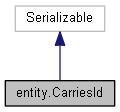
\includegraphics[width=162pt]{classentity_1_1_carries_id__inherit__graph}
\end{center}
\end{figure}


Collaboration diagram for entity.\+Carries\+Id\+:\nopagebreak
\begin{figure}[H]
\begin{center}
\leavevmode
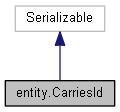
\includegraphics[width=162pt]{classentity_1_1_carries_id__coll__graph}
\end{center}
\end{figure}
\subsection*{Public Member Functions}
\begin{DoxyCompactItemize}
\item 
\mbox{\Hypertarget{classentity_1_1_carries_id_a51dae5e60540dcdb4b5c4a5c59ce8aed}\label{classentity_1_1_carries_id_a51dae5e60540dcdb4b5c4a5c59ce8aed}} 
{\bfseries Carries\+Id} (byte order\+Product\+Id)
\item 
\mbox{\Hypertarget{classentity_1_1_carries_id_a3c7555deb455253a857ecb72a99c0c1e}\label{classentity_1_1_carries_id_a3c7555deb455253a857ecb72a99c0c1e}} 
{\bfseries Carries\+Id} (byte order\+Product\+Id, Byte initial\+Workstation\+Id, Byte destiny\+Workstation\+Id, Byte machine\+Id, Boolean state)
\item 
\mbox{\Hypertarget{classentity_1_1_carries_id_a774d57bdffd816d281e67bd06bf62d21}\label{classentity_1_1_carries_id_a774d57bdffd816d281e67bd06bf62d21}} 
int {\bfseries get\+Order\+Product\+Id} ()
\item 
\mbox{\Hypertarget{classentity_1_1_carries_id_a9049878112d9a3423f96ea5593afeb6f}\label{classentity_1_1_carries_id_a9049878112d9a3423f96ea5593afeb6f}} 
void {\bfseries set\+Order\+Product\+Id} (int order\+Product\+Id)
\item 
\mbox{\Hypertarget{classentity_1_1_carries_id_a9f0d4a30dbe0db09bab463393bd6d1f5}\label{classentity_1_1_carries_id_a9f0d4a30dbe0db09bab463393bd6d1f5}} 
Byte {\bfseries get\+Initial\+Workstation\+Id} ()
\item 
\mbox{\Hypertarget{classentity_1_1_carries_id_a2f055c85f701e12e2d93e054189414c6}\label{classentity_1_1_carries_id_a2f055c85f701e12e2d93e054189414c6}} 
void {\bfseries set\+Initial\+Workstation\+Id} (Byte initial\+Workstation\+Id)
\item 
\mbox{\Hypertarget{classentity_1_1_carries_id_a6806d0507a1e0e67cc2cb3668255a1b8}\label{classentity_1_1_carries_id_a6806d0507a1e0e67cc2cb3668255a1b8}} 
Byte {\bfseries get\+Destiny\+Workstation\+Id} ()
\item 
\mbox{\Hypertarget{classentity_1_1_carries_id_af9516f9d5e88954e3e72457f2ccf4f7b}\label{classentity_1_1_carries_id_af9516f9d5e88954e3e72457f2ccf4f7b}} 
void {\bfseries set\+Destiny\+Workstation\+Id} (Byte destiny\+Workstation\+Id)
\item 
\mbox{\Hypertarget{classentity_1_1_carries_id_a625fe262ed6c802bc07f9f4cc4a989bb}\label{classentity_1_1_carries_id_a625fe262ed6c802bc07f9f4cc4a989bb}} 
Byte {\bfseries get\+Machine\+Id} ()
\item 
\mbox{\Hypertarget{classentity_1_1_carries_id_aa5bba6ca3cb097ea91354987f1b6a2f0}\label{classentity_1_1_carries_id_aa5bba6ca3cb097ea91354987f1b6a2f0}} 
void {\bfseries set\+Machine\+Id} (Byte machine\+Id)
\item 
\mbox{\Hypertarget{classentity_1_1_carries_id_a123b2805042dd0fe551c2e766b961129}\label{classentity_1_1_carries_id_a123b2805042dd0fe551c2e766b961129}} 
Boolean {\bfseries get\+State} ()
\item 
\mbox{\Hypertarget{classentity_1_1_carries_id_a8f8f0f103d2fd8db15b6416370d690e1}\label{classentity_1_1_carries_id_a8f8f0f103d2fd8db15b6416370d690e1}} 
void {\bfseries set\+State} (Boolean state)
\item 
\mbox{\Hypertarget{classentity_1_1_carries_id_ac343763b0821ae53aa653fc269cb0172}\label{classentity_1_1_carries_id_ac343763b0821ae53aa653fc269cb0172}} 
boolean {\bfseries equals} (Object other)
\item 
\mbox{\Hypertarget{classentity_1_1_carries_id_a2d5ebee74ab620ab24e2ab3da501cfd9}\label{classentity_1_1_carries_id_a2d5ebee74ab620ab24e2ab3da501cfd9}} 
int {\bfseries hash\+Code} ()
\end{DoxyCompactItemize}


\subsection{Detailed Description}
\mbox{\hyperlink{classentity_1_1_carries_id}{Carries\+Id}} generated by hbm2java 

The documentation for this class was generated from the following file\+:\begin{DoxyCompactItemize}
\item 
src/main/java/entity/Carries\+Id.\+java\end{DoxyCompactItemize}

\hypertarget{classcontroller_1_1_customer_controller}{}\section{controller.\+Customer\+Controller Class Reference}
\label{classcontroller_1_1_customer_controller}\index{controller.\+Customer\+Controller@{controller.\+Customer\+Controller}}


Collaboration diagram for controller.\+Customer\+Controller\+:\nopagebreak
\begin{figure}[H]
\begin{center}
\leavevmode
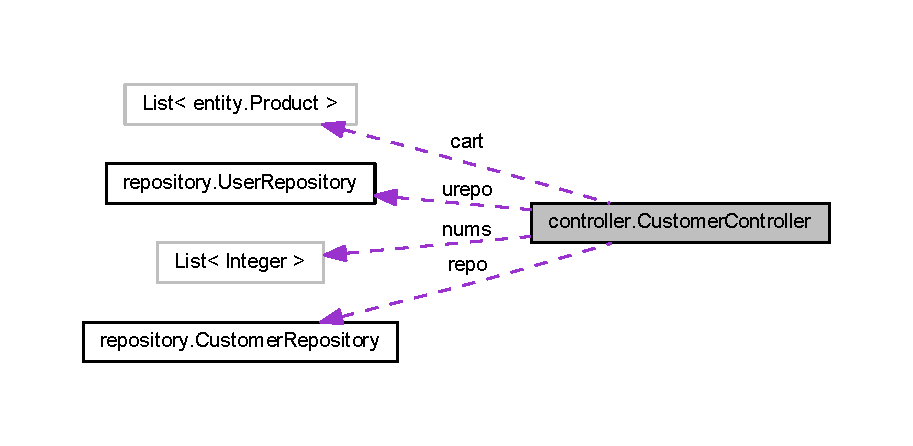
\includegraphics[width=350pt]{classcontroller_1_1_customer_controller__coll__graph}
\end{center}
\end{figure}
\subsection*{Public Member Functions}
\begin{DoxyCompactItemize}
\item 
String \mbox{\hyperlink{classcontroller_1_1_customer_controller_a5496f4bf5f03f585ee223c0192d4fc85}{customer}} (Model m, Web\+Request request, Http\+Servlet\+Response response, Http\+Servlet\+Request hrequest)  throws I\+O\+Exception 
\item 
String \mbox{\hyperlink{classcontroller_1_1_customer_controller_a9c7aebe2a5ae4e7419fd10121a6a7189}{show\+Product}} (Model m, Web\+Request request, Http\+Servlet\+Response response, Http\+Servlet\+Request hrequest)  throws I\+O\+Exception 
\item 
String \mbox{\hyperlink{classcontroller_1_1_customer_controller_af47f965b533083f4415c63f1065cbd64}{orders}} (Model m, Web\+Request request, Http\+Servlet\+Request hrequest, Http\+Servlet\+Response response)  throws I\+O\+Exception 
\item 
String \mbox{\hyperlink{classcontroller_1_1_customer_controller_a74ff447f25dce313f84a08cf5356f8e8}{order}} (Model m, Web\+Request request)
\item 
String \mbox{\hyperlink{classcontroller_1_1_customer_controller_a90aa906ff9e90be62b82941992350235}{cart}} (Model m, Web\+Request request, Http\+Servlet\+Request hrequest, Http\+Servlet\+Response response)  throws I\+O\+Exception 
\item 
String \mbox{\hyperlink{classcontroller_1_1_customer_controller_add866b64d6e08876db8b97087eaeb389}{chart}} (Model m, Web\+Request request)
\end{DoxyCompactItemize}


\subsection{Detailed Description}
\mbox{\hyperlink{classcontroller_1_1_customer_controller}{Customer\+Controller}} contains the U\+RL actions of the Customer user type

\begin{DoxyAuthor}{Author}
Leire 
\end{DoxyAuthor}


\subsection{Member Function Documentation}
\mbox{\Hypertarget{classcontroller_1_1_customer_controller_a90aa906ff9e90be62b82941992350235}\label{classcontroller_1_1_customer_controller_a90aa906ff9e90be62b82941992350235}} 
\index{controller\+::\+Customer\+Controller@{controller\+::\+Customer\+Controller}!cart@{cart}}
\index{cart@{cart}!controller\+::\+Customer\+Controller@{controller\+::\+Customer\+Controller}}
\subsubsection{\texorpdfstring{cart()}{cart()}}
{\footnotesize\ttfamily String controller.\+Customer\+Controller.\+cart (\begin{DoxyParamCaption}\item[{Model}]{m,  }\item[{Web\+Request}]{request,  }\item[{Http\+Servlet\+Request}]{hrequest,  }\item[{Http\+Servlet\+Response}]{response }\end{DoxyParamCaption}) throws I\+O\+Exception\hspace{0.3cm}{\ttfamily [inline]}}

This method will show the actual cart of the customer 
\begin{DoxyExceptions}{Exceptions}
{\em I\+O\+Exception} & \\
\hline
\end{DoxyExceptions}
\mbox{\Hypertarget{classcontroller_1_1_customer_controller_add866b64d6e08876db8b97087eaeb389}\label{classcontroller_1_1_customer_controller_add866b64d6e08876db8b97087eaeb389}} 
\index{controller\+::\+Customer\+Controller@{controller\+::\+Customer\+Controller}!chart@{chart}}
\index{chart@{chart}!controller\+::\+Customer\+Controller@{controller\+::\+Customer\+Controller}}
\subsubsection{\texorpdfstring{chart()}{chart()}}
{\footnotesize\ttfamily String controller.\+Customer\+Controller.\+chart (\begin{DoxyParamCaption}\item[{Model}]{m,  }\item[{Web\+Request}]{request }\end{DoxyParamCaption})\hspace{0.3cm}{\ttfamily [inline]}}

This method will show a chart showing the history of the products bought by the customer \mbox{\Hypertarget{classcontroller_1_1_customer_controller_a5496f4bf5f03f585ee223c0192d4fc85}\label{classcontroller_1_1_customer_controller_a5496f4bf5f03f585ee223c0192d4fc85}} 
\index{controller\+::\+Customer\+Controller@{controller\+::\+Customer\+Controller}!customer@{customer}}
\index{customer@{customer}!controller\+::\+Customer\+Controller@{controller\+::\+Customer\+Controller}}
\subsubsection{\texorpdfstring{customer()}{customer()}}
{\footnotesize\ttfamily String controller.\+Customer\+Controller.\+customer (\begin{DoxyParamCaption}\item[{Model}]{m,  }\item[{Web\+Request}]{request,  }\item[{Http\+Servlet\+Response}]{response,  }\item[{Http\+Servlet\+Request}]{hrequest }\end{DoxyParamCaption}) throws I\+O\+Exception\hspace{0.3cm}{\ttfamily [inline]}}

This method will access the customer\textquotesingle{}s main site. Here, the customer will be able to see all the products available on the store. 
\begin{DoxyExceptions}{Exceptions}
{\em I\+O\+Exception} & \\
\hline
\end{DoxyExceptions}
\mbox{\Hypertarget{classcontroller_1_1_customer_controller_a74ff447f25dce313f84a08cf5356f8e8}\label{classcontroller_1_1_customer_controller_a74ff447f25dce313f84a08cf5356f8e8}} 
\index{controller\+::\+Customer\+Controller@{controller\+::\+Customer\+Controller}!order@{order}}
\index{order@{order}!controller\+::\+Customer\+Controller@{controller\+::\+Customer\+Controller}}
\subsubsection{\texorpdfstring{order()}{order()}}
{\footnotesize\ttfamily String controller.\+Customer\+Controller.\+order (\begin{DoxyParamCaption}\item[{Model}]{m,  }\item[{Web\+Request}]{request }\end{DoxyParamCaption})\hspace{0.3cm}{\ttfamily [inline]}}

This method will access the customer\textquotesingle{}s \textquotesingle{}orders\textquotesingle{} option, where the customer will be able to seea concrete order. \mbox{\Hypertarget{classcontroller_1_1_customer_controller_af47f965b533083f4415c63f1065cbd64}\label{classcontroller_1_1_customer_controller_af47f965b533083f4415c63f1065cbd64}} 
\index{controller\+::\+Customer\+Controller@{controller\+::\+Customer\+Controller}!orders@{orders}}
\index{orders@{orders}!controller\+::\+Customer\+Controller@{controller\+::\+Customer\+Controller}}
\subsubsection{\texorpdfstring{orders()}{orders()}}
{\footnotesize\ttfamily String controller.\+Customer\+Controller.\+orders (\begin{DoxyParamCaption}\item[{Model}]{m,  }\item[{Web\+Request}]{request,  }\item[{Http\+Servlet\+Request}]{hrequest,  }\item[{Http\+Servlet\+Response}]{response }\end{DoxyParamCaption}) throws I\+O\+Exception\hspace{0.3cm}{\ttfamily [inline]}}

This method will access the customer\textquotesingle{}s \textquotesingle{}orders\textquotesingle{} option, where the customer will be able to see the orders made through their history. 
\begin{DoxyExceptions}{Exceptions}
{\em I\+O\+Exception} & \\
\hline
\end{DoxyExceptions}
\mbox{\Hypertarget{classcontroller_1_1_customer_controller_a9c7aebe2a5ae4e7419fd10121a6a7189}\label{classcontroller_1_1_customer_controller_a9c7aebe2a5ae4e7419fd10121a6a7189}} 
\index{controller\+::\+Customer\+Controller@{controller\+::\+Customer\+Controller}!show\+Product@{show\+Product}}
\index{show\+Product@{show\+Product}!controller\+::\+Customer\+Controller@{controller\+::\+Customer\+Controller}}
\subsubsection{\texorpdfstring{show\+Product()}{showProduct()}}
{\footnotesize\ttfamily String controller.\+Customer\+Controller.\+show\+Product (\begin{DoxyParamCaption}\item[{Model}]{m,  }\item[{Web\+Request}]{request,  }\item[{Http\+Servlet\+Response}]{response,  }\item[{Http\+Servlet\+Request}]{hrequest }\end{DoxyParamCaption}) throws I\+O\+Exception\hspace{0.3cm}{\ttfamily [inline]}}

This method will access the customer\textquotesingle{}s \textquotesingle{}products\textquotesingle{} option, where the customer will be able to see all the products available on the store. 
\begin{DoxyExceptions}{Exceptions}
{\em I\+O\+Exception} & \\
\hline
\end{DoxyExceptions}


The documentation for this class was generated from the following file\+:\begin{DoxyCompactItemize}
\item 
src/main/java/controller/Customer\+Controller.\+java\end{DoxyCompactItemize}

\hypertarget{classentity_1_1_departament}{}\section{entity.\+Departament Class Reference}
\label{classentity_1_1_departament}\index{entity.\+Departament@{entity.\+Departament}}


Inheritance diagram for entity.\+Departament\+:
% FIG 0


Collaboration diagram for entity.\+Departament\+:
% FIG 1
\subsection*{Public Member Functions}
\begin{DoxyCompactItemize}
\item 
\mbox{\Hypertarget{classentity_1_1_departament_aabee9c9d6e8ebac494a04b155b1dc88b}\label{classentity_1_1_departament_aabee9c9d6e8ebac494a04b155b1dc88b}} 
{\bfseries Departament} (byte departament\+Id, String dep\+Name)
\item 
\mbox{\Hypertarget{classentity_1_1_departament_a54014ddb3c17c6a16b30c6b3ca8bc5f7}\label{classentity_1_1_departament_a54014ddb3c17c6a16b30c6b3ca8bc5f7}} 
{\bfseries Departament} (byte departament\+Id, String dep\+Name, String description, Set products)
\item 
\mbox{\Hypertarget{classentity_1_1_departament_ab1c66ffc4862ab88d0f49a85f5358b4c}\label{classentity_1_1_departament_ab1c66ffc4862ab88d0f49a85f5358b4c}} 
byte {\bfseries get\+Departament\+Id} ()
\item 
\mbox{\Hypertarget{classentity_1_1_departament_a35cf439bb17df38af5f4d7dbcfb6413b}\label{classentity_1_1_departament_a35cf439bb17df38af5f4d7dbcfb6413b}} 
void {\bfseries set\+Departament\+Id} (byte departament\+Id)
\item 
\mbox{\Hypertarget{classentity_1_1_departament_a28c9949df7e14641133dcca20f5562dc}\label{classentity_1_1_departament_a28c9949df7e14641133dcca20f5562dc}} 
String {\bfseries get\+Dep\+Name} ()
\item 
\mbox{\Hypertarget{classentity_1_1_departament_aea77ef1f0c423cdde3317cc47a2f37b7}\label{classentity_1_1_departament_aea77ef1f0c423cdde3317cc47a2f37b7}} 
void {\bfseries set\+Dep\+Name} (String dep\+Name)
\item 
\mbox{\Hypertarget{classentity_1_1_departament_a5332bf92f5b29d56e9559037f3c6f4a2}\label{classentity_1_1_departament_a5332bf92f5b29d56e9559037f3c6f4a2}} 
String {\bfseries get\+Description} ()
\item 
\mbox{\Hypertarget{classentity_1_1_departament_a4ffc7e3a45ab3a5878e3c1fa65695078}\label{classentity_1_1_departament_a4ffc7e3a45ab3a5878e3c1fa65695078}} 
void {\bfseries set\+Description} (String description)
\item 
\mbox{\Hypertarget{classentity_1_1_departament_a54994f6d08777e9a90cb8ca2afe7c424}\label{classentity_1_1_departament_a54994f6d08777e9a90cb8ca2afe7c424}} 
Set {\bfseries get\+Products} ()
\item 
\mbox{\Hypertarget{classentity_1_1_departament_a35fb7482cd77c6b83765606724be74b6}\label{classentity_1_1_departament_a35fb7482cd77c6b83765606724be74b6}} 
void {\bfseries set\+Products} (Set products)
\end{DoxyCompactItemize}


\subsection{Detailed Description}
\mbox{\hyperlink{classentity_1_1_departament}{Departament}} generated by hbm2java 

The documentation for this class was generated from the following file\+:\begin{DoxyCompactItemize}
\item 
D\+:/\+Users/user/\+Documents/\+M\+O\+N\+D\+R\+A/3.\+M\+A\+I\+L\+A/\+P\+O\+P\+B\+L5/\+Programak/e\+Jkiva\+\_\+\+P\+O\+P\+B\+L5/\+Web application workspace/e\+Jkiva/src/main/java/entity/Departament.\+java\end{DoxyCompactItemize}

\hypertarget{classutils_1_1_hibernate_utils}{}\section{utils.\+Hibernate\+Utils Class Reference}
\label{classutils_1_1_hibernate_utils}\index{utils.\+Hibernate\+Utils@{utils.\+Hibernate\+Utils}}
\subsection*{Static Public Member Functions}
\begin{DoxyCompactItemize}
\item 
\mbox{\Hypertarget{classutils_1_1_hibernate_utils_a48f212775a4d87ceb1116c11f05d4053}\label{classutils_1_1_hibernate_utils_a48f212775a4d87ceb1116c11f05d4053}} 
static Session\+Factory {\bfseries get\+Session\+Factory} ()
\end{DoxyCompactItemize}


The documentation for this class was generated from the following file\+:\begin{DoxyCompactItemize}
\item 
D\+:/\+Users/user/\+Documents/\+M\+O\+N\+D\+R\+A/3.\+M\+A\+I\+L\+A/\+P\+O\+P\+B\+L5/\+Programak/e\+Jkiva\+\_\+\+P\+O\+P\+B\+L5/\+Web application workspace/e\+Jkiva/src/main/java/utils/Hibernate\+Utils.\+java\end{DoxyCompactItemize}

\hypertarget{classcontroller_1_1_login_controller}{}\section{controller.\+Login\+Controller Class Reference}
\label{classcontroller_1_1_login_controller}\index{controller.\+Login\+Controller@{controller.\+Login\+Controller}}


Collaboration diagram for controller.\+Login\+Controller\+:\nopagebreak
\begin{figure}[H]
\begin{center}
\leavevmode
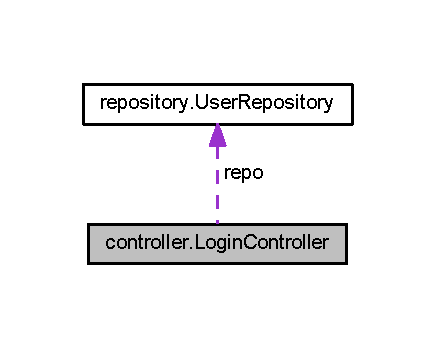
\includegraphics[width=209pt]{classcontroller_1_1_login_controller__coll__graph}
\end{center}
\end{figure}
\subsection*{Public Member Functions}
\begin{DoxyCompactItemize}
\item 
String \mbox{\hyperlink{classcontroller_1_1_login_controller_a98e670c0e2a6a391f1b5b9cb451aedeb}{login}} (Model m, Http\+Servlet\+Response response, Http\+Servlet\+Request request, Web\+Request wrequest)  throws Exception 
\end{DoxyCompactItemize}


\subsection{Detailed Description}
Login class.

\begin{DoxyAuthor}{Author}
Leire 
\end{DoxyAuthor}


\subsection{Member Function Documentation}
\mbox{\Hypertarget{classcontroller_1_1_login_controller_a98e670c0e2a6a391f1b5b9cb451aedeb}\label{classcontroller_1_1_login_controller_a98e670c0e2a6a391f1b5b9cb451aedeb}} 
\index{controller\+::\+Login\+Controller@{controller\+::\+Login\+Controller}!login@{login}}
\index{login@{login}!controller\+::\+Login\+Controller@{controller\+::\+Login\+Controller}}
\subsubsection{\texorpdfstring{login()}{login()}}
{\footnotesize\ttfamily String controller.\+Login\+Controller.\+login (\begin{DoxyParamCaption}\item[{Model}]{m,  }\item[{Http\+Servlet\+Response}]{response,  }\item[{Http\+Servlet\+Request}]{request,  }\item[{Web\+Request}]{wrequest }\end{DoxyParamCaption}) throws Exception\hspace{0.3cm}{\ttfamily [inline]}}

This method will login or register a user and redirect them depending on their type 
\begin{DoxyExceptions}{Exceptions}
{\em Exception} & \\
\hline
\end{DoxyExceptions}


The documentation for this class was generated from the following file\+:\begin{DoxyCompactItemize}
\item 
src/main/java/controller/Login\+Controller.\+java\end{DoxyCompactItemize}

\hypertarget{classentity_1_1_order}{}\section{entity.\+Order Class Reference}
\label{classentity_1_1_order}\index{entity.\+Order@{entity.\+Order}}


Inheritance diagram for entity.\+Order\+:\nopagebreak
\begin{figure}[H]
\begin{center}
\leavevmode
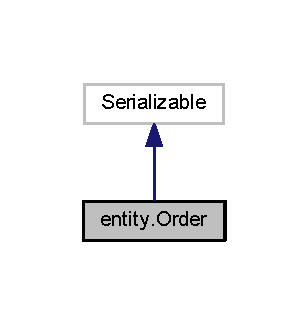
\includegraphics[width=148pt]{classentity_1_1_order__inherit__graph}
\end{center}
\end{figure}


Collaboration diagram for entity.\+Order\+:\nopagebreak
\begin{figure}[H]
\begin{center}
\leavevmode
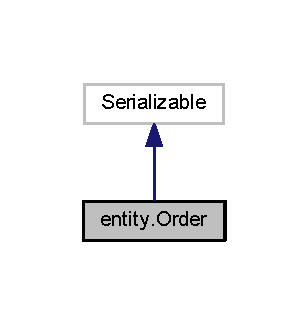
\includegraphics[width=148pt]{classentity_1_1_order__coll__graph}
\end{center}
\end{figure}
\subsection*{Public Member Functions}
\begin{DoxyCompactItemize}
\item 
\mbox{\Hypertarget{classentity_1_1_order_a29eb9dead0b1577bd57bc3a5db15f981}\label{classentity_1_1_order_a29eb9dead0b1577bd57bc3a5db15f981}} 
{\bfseries Order} (\mbox{\hyperlink{classentity_1_1_user}{User}} user, Date date\+Order)
\item 
\mbox{\Hypertarget{classentity_1_1_order_a5180af95fecce83f0416706550fed72d}\label{classentity_1_1_order_a5180af95fecce83f0416706550fed72d}} 
{\bfseries Order} (\mbox{\hyperlink{classentity_1_1_user}{User}} user, Date date\+Order, Date date\+Delivered)
\item 
\mbox{\Hypertarget{classentity_1_1_order_a4561af92f26502434e496c32164ea1ff}\label{classentity_1_1_order_a4561af92f26502434e496c32164ea1ff}} 
int {\bfseries get\+Order\+Id} ()
\item 
\mbox{\Hypertarget{classentity_1_1_order_a780f89a2c6102d22cc7c076b7a038c8f}\label{classentity_1_1_order_a780f89a2c6102d22cc7c076b7a038c8f}} 
void {\bfseries set\+Order\+Id} (int order\+Id)
\item 
\mbox{\Hypertarget{classentity_1_1_order_a5262114e6d86f0826384b5aebaa04856}\label{classentity_1_1_order_a5262114e6d86f0826384b5aebaa04856}} 
\mbox{\hyperlink{classentity_1_1_user}{User}} {\bfseries get\+User} ()
\item 
\mbox{\Hypertarget{classentity_1_1_order_ad8de4f52695d2a9230e9bdb0aa42decb}\label{classentity_1_1_order_ad8de4f52695d2a9230e9bdb0aa42decb}} 
void {\bfseries set\+User} (\mbox{\hyperlink{classentity_1_1_user}{User}} user)
\item 
\mbox{\Hypertarget{classentity_1_1_order_a69a26d54af50e17b399f6af80433b569}\label{classentity_1_1_order_a69a26d54af50e17b399f6af80433b569}} 
Date {\bfseries get\+Date\+Order} ()
\item 
\mbox{\Hypertarget{classentity_1_1_order_a0c2fee67a9b341a27e83b875534bf9ea}\label{classentity_1_1_order_a0c2fee67a9b341a27e83b875534bf9ea}} 
void {\bfseries set\+Date\+Order} (Date date\+Order)
\item 
\mbox{\Hypertarget{classentity_1_1_order_a949fad3af9e1747db36124d934ed6413}\label{classentity_1_1_order_a949fad3af9e1747db36124d934ed6413}} 
Date {\bfseries get\+Date\+Delivered} ()
\item 
\mbox{\Hypertarget{classentity_1_1_order_a36942ca27b3ac8f905319ba13986ff19}\label{classentity_1_1_order_a36942ca27b3ac8f905319ba13986ff19}} 
void {\bfseries set\+Date\+Delivered} (Date date\+Delivered)
\end{DoxyCompactItemize}


\subsection{Detailed Description}
\mbox{\hyperlink{classentity_1_1_order}{Order}} generated by hbm2java 

The documentation for this class was generated from the following file\+:\begin{DoxyCompactItemize}
\item 
src/main/java/entity/Order.\+java\end{DoxyCompactItemize}

\hypertarget{classentity_1_1_orderproduct}{}\section{entity.\+Orderproduct Class Reference}
\label{classentity_1_1_orderproduct}\index{entity.\+Orderproduct@{entity.\+Orderproduct}}


Inheritance diagram for entity.\+Orderproduct\+:
% FIG 0


Collaboration diagram for entity.\+Orderproduct\+:
% FIG 1
\subsection*{Public Member Functions}
\begin{DoxyCompactItemize}
\item 
\mbox{\Hypertarget{classentity_1_1_orderproduct_a141723329278c6424a1d300db29529a4}\label{classentity_1_1_orderproduct_a141723329278c6424a1d300db29529a4}} 
{\bfseries Orderproduct} (\mbox{\hyperlink{classentity_1_1_order}{Order}} order, \mbox{\hyperlink{classentity_1_1_product}{Product}} product, short quantity)
\item 
\mbox{\Hypertarget{classentity_1_1_orderproduct_a08d3bfc82478033cba0386026800358b}\label{classentity_1_1_orderproduct_a08d3bfc82478033cba0386026800358b}} 
int {\bfseries get\+Order\+Product\+Id} ()
\item 
\mbox{\Hypertarget{classentity_1_1_orderproduct_afb5336d8fb886081876eb8b69970daad}\label{classentity_1_1_orderproduct_afb5336d8fb886081876eb8b69970daad}} 
void {\bfseries set\+Order\+Product\+Id} (int order\+Product\+Id)
\item 
\mbox{\Hypertarget{classentity_1_1_orderproduct_af160d989a7a8c448ce983743a8ee1578}\label{classentity_1_1_orderproduct_af160d989a7a8c448ce983743a8ee1578}} 
\mbox{\hyperlink{classentity_1_1_order}{Order}} {\bfseries get\+Order} ()
\item 
\mbox{\Hypertarget{classentity_1_1_orderproduct_ac38152f038c0669a8f2280c6f55fc1bb}\label{classentity_1_1_orderproduct_ac38152f038c0669a8f2280c6f55fc1bb}} 
void {\bfseries set\+Order} (\mbox{\hyperlink{classentity_1_1_order}{Order}} order)
\item 
\mbox{\Hypertarget{classentity_1_1_orderproduct_ac8a5d534f8433a8260ea87a85bb00217}\label{classentity_1_1_orderproduct_ac8a5d534f8433a8260ea87a85bb00217}} 
\mbox{\hyperlink{classentity_1_1_product}{Product}} {\bfseries get\+Product} ()
\item 
\mbox{\Hypertarget{classentity_1_1_orderproduct_a4d9fd082a96c982443e6ad4cfb032a61}\label{classentity_1_1_orderproduct_a4d9fd082a96c982443e6ad4cfb032a61}} 
void {\bfseries set\+Product} (\mbox{\hyperlink{classentity_1_1_product}{Product}} product)
\item 
\mbox{\Hypertarget{classentity_1_1_orderproduct_a4a10cb8ecd7ac4c692f5f3fa96793e9d}\label{classentity_1_1_orderproduct_a4a10cb8ecd7ac4c692f5f3fa96793e9d}} 
short {\bfseries get\+Quantity} ()
\item 
\mbox{\Hypertarget{classentity_1_1_orderproduct_ab402591f6605ff9ad60a62175b4e6d0d}\label{classentity_1_1_orderproduct_ab402591f6605ff9ad60a62175b4e6d0d}} 
void {\bfseries set\+Quantity} (short quantity)
\end{DoxyCompactItemize}


\subsection{Detailed Description}
\mbox{\hyperlink{classentity_1_1_orderproduct}{Orderproduct}} generated by hbm2java 

The documentation for this class was generated from the following file\+:\begin{DoxyCompactItemize}
\item 
D\+:/\+Users/user/\+Documents/\+M\+O\+N\+D\+R\+A/3.\+M\+A\+I\+L\+A/\+P\+O\+P\+B\+L5/\+G\+I\+T/e\+Jkiva\+\_\+\+P\+O\+P\+B\+L5/e\+Jkiva/src/main/java/entity/Orderproduct.\+java\end{DoxyCompactItemize}

\hypertarget{classentity_1_1_product}{}\section{entity.\+Product Class Reference}
\label{classentity_1_1_product}\index{entity.\+Product@{entity.\+Product}}


Inheritance diagram for entity.\+Product\+:
% FIG 0


Collaboration diagram for entity.\+Product\+:
% FIG 1
\subsection*{Public Member Functions}
\begin{DoxyCompactItemize}
\item 
\mbox{\Hypertarget{classentity_1_1_product_a16490d212d113e14eb833a18ffd35c9e}\label{classentity_1_1_product_a16490d212d113e14eb833a18ffd35c9e}} 
{\bfseries Product} (String product\+Name, float price)
\item 
\mbox{\Hypertarget{classentity_1_1_product_aac8d06cb1b251960fd960abec0ed08ce}\label{classentity_1_1_product_aac8d06cb1b251960fd960abec0ed08ce}} 
{\bfseries Product} (\mbox{\hyperlink{classentity_1_1_departament}{Departament}} departament, String product\+Name, String description, float price, String image)
\item 
\mbox{\Hypertarget{classentity_1_1_product_a2d097a6e21ca5384407ef2d5629409d0}\label{classentity_1_1_product_a2d097a6e21ca5384407ef2d5629409d0}} 
int {\bfseries get\+Product\+Id} ()
\item 
\mbox{\Hypertarget{classentity_1_1_product_ad9a9458cf69f508b1d80cd90f4649343}\label{classentity_1_1_product_ad9a9458cf69f508b1d80cd90f4649343}} 
void {\bfseries set\+Product\+Id} (int product\+Id)
\item 
\mbox{\Hypertarget{classentity_1_1_product_a78bd5ae5f85a3d22bdd23b84c07f1ed4}\label{classentity_1_1_product_a78bd5ae5f85a3d22bdd23b84c07f1ed4}} 
\mbox{\hyperlink{classentity_1_1_departament}{Departament}} {\bfseries get\+Departament} ()
\item 
\mbox{\Hypertarget{classentity_1_1_product_aa67771d630e8eb1922b751a266df6a62}\label{classentity_1_1_product_aa67771d630e8eb1922b751a266df6a62}} 
void {\bfseries set\+Departament} (\mbox{\hyperlink{classentity_1_1_departament}{Departament}} departament)
\item 
\mbox{\Hypertarget{classentity_1_1_product_a81d43916d1f7b73a2f087e3570d73de0}\label{classentity_1_1_product_a81d43916d1f7b73a2f087e3570d73de0}} 
String {\bfseries get\+Product\+Name} ()
\item 
\mbox{\Hypertarget{classentity_1_1_product_abbed2e3b34beb9eff42595b8e2641f7a}\label{classentity_1_1_product_abbed2e3b34beb9eff42595b8e2641f7a}} 
void {\bfseries set\+Product\+Name} (String product\+Name)
\item 
\mbox{\Hypertarget{classentity_1_1_product_a33ba8df9ce2e2cbf6091bb97a0ee0f2c}\label{classentity_1_1_product_a33ba8df9ce2e2cbf6091bb97a0ee0f2c}} 
String {\bfseries get\+Description} ()
\item 
\mbox{\Hypertarget{classentity_1_1_product_a275f824222328131f6a00f383196da41}\label{classentity_1_1_product_a275f824222328131f6a00f383196da41}} 
void {\bfseries set\+Description} (String description)
\item 
\mbox{\Hypertarget{classentity_1_1_product_af6bbc7b34e0ab7b7f2fe758d174fa5f4}\label{classentity_1_1_product_af6bbc7b34e0ab7b7f2fe758d174fa5f4}} 
float {\bfseries get\+Price} ()
\item 
\mbox{\Hypertarget{classentity_1_1_product_a096085200f5ea9730661bc114a0f929d}\label{classentity_1_1_product_a096085200f5ea9730661bc114a0f929d}} 
void {\bfseries set\+Price} (float price)
\item 
\mbox{\Hypertarget{classentity_1_1_product_a5466888d66016874eb475a2703cbc709}\label{classentity_1_1_product_a5466888d66016874eb475a2703cbc709}} 
String {\bfseries get\+Image} ()
\item 
\mbox{\Hypertarget{classentity_1_1_product_a02b293f40f4d82e30617fdc2be6fac49}\label{classentity_1_1_product_a02b293f40f4d82e30617fdc2be6fac49}} 
void {\bfseries set\+Image} (String image)
\item 
\mbox{\Hypertarget{classentity_1_1_product_ad77da4f2b6b67974fd2a040e2b930970}\label{classentity_1_1_product_ad77da4f2b6b67974fd2a040e2b930970}} 
String {\bfseries to\+String} ()
\end{DoxyCompactItemize}


\subsection{Detailed Description}
\mbox{\hyperlink{classentity_1_1_product}{Product}} generated by hbm2java 

The documentation for this class was generated from the following file\+:\begin{DoxyCompactItemize}
\item 
D\+:/\+Users/user/\+Documents/\+M\+O\+N\+D\+R\+A/3.\+M\+A\+I\+L\+A/\+P\+O\+P\+B\+L5/\+G\+I\+T/e\+Jkiva\+\_\+\+P\+O\+P\+B\+L5/e\+Jkiva/src/main/java/entity/Product.\+java\end{DoxyCompactItemize}

\hypertarget{classentity_1_1_segment}{}\section{entity.\+Segment Class Reference}
\label{classentity_1_1_segment}\index{entity.\+Segment@{entity.\+Segment}}


Inheritance diagram for entity.\+Segment\+:
% FIG 0


Collaboration diagram for entity.\+Segment\+:
% FIG 1
\subsection*{Public Member Functions}
\begin{DoxyCompactItemize}
\item 
\mbox{\Hypertarget{classentity_1_1_segment_a4198d8bf80daca7aec679e294b962f28}\label{classentity_1_1_segment_a4198d8bf80daca7aec679e294b962f28}} 
{\bfseries Segment} (String segment, short posX, short posY)
\item 
\mbox{\Hypertarget{classentity_1_1_segment_a7d23189c239956e9a6580bab38b4dab1}\label{classentity_1_1_segment_a7d23189c239956e9a6580bab38b4dab1}} 
{\bfseries Segment} (String segment, short posX, short posY, String description, Set authomaches, Set workstations)
\item 
\mbox{\Hypertarget{classentity_1_1_segment_a1e00c79b38639370d9b116a6c77a5b4a}\label{classentity_1_1_segment_a1e00c79b38639370d9b116a6c77a5b4a}} 
int {\bfseries get\+Segment\+Id} ()
\item 
\mbox{\Hypertarget{classentity_1_1_segment_a49190cea3afa331fe0c5fbc10e6214ec}\label{classentity_1_1_segment_a49190cea3afa331fe0c5fbc10e6214ec}} 
void {\bfseries set\+Segment\+Id} (Byte segment\+Id)
\item 
\mbox{\Hypertarget{classentity_1_1_segment_af96f1caaaaf411990b64270c830c3456}\label{classentity_1_1_segment_af96f1caaaaf411990b64270c830c3456}} 
String {\bfseries get\+Segment} ()
\item 
\mbox{\Hypertarget{classentity_1_1_segment_abb149147dc902ee032e3bff790010cec}\label{classentity_1_1_segment_abb149147dc902ee032e3bff790010cec}} 
void {\bfseries set\+Segment} (String segment)
\item 
\mbox{\Hypertarget{classentity_1_1_segment_a0c740639c2fb9fc93add3e63adb4879a}\label{classentity_1_1_segment_a0c740639c2fb9fc93add3e63adb4879a}} 
short {\bfseries get\+PosX} ()
\item 
\mbox{\Hypertarget{classentity_1_1_segment_a8a0c1e5d9ccefcefe2fd5d28ff5703dd}\label{classentity_1_1_segment_a8a0c1e5d9ccefcefe2fd5d28ff5703dd}} 
void {\bfseries set\+PosX} (short posX)
\item 
\mbox{\Hypertarget{classentity_1_1_segment_a49e9f7232f10a5d429f82782a96be138}\label{classentity_1_1_segment_a49e9f7232f10a5d429f82782a96be138}} 
short {\bfseries get\+PosY} ()
\item 
\mbox{\Hypertarget{classentity_1_1_segment_a6ce06e8e4f24903d09ae2c73505035d0}\label{classentity_1_1_segment_a6ce06e8e4f24903d09ae2c73505035d0}} 
void {\bfseries set\+PosY} (short posY)
\item 
\mbox{\Hypertarget{classentity_1_1_segment_a8ac2a6c8d6e1948962c6dd6090c0fe36}\label{classentity_1_1_segment_a8ac2a6c8d6e1948962c6dd6090c0fe36}} 
String {\bfseries get\+Description} ()
\item 
\mbox{\Hypertarget{classentity_1_1_segment_a7bea5d3fe2bc567b8f1b66c352a60b1c}\label{classentity_1_1_segment_a7bea5d3fe2bc567b8f1b66c352a60b1c}} 
void {\bfseries set\+Description} (String description)
\item 
\mbox{\Hypertarget{classentity_1_1_segment_a292b54976ba0f33d4e044cc19c11392a}\label{classentity_1_1_segment_a292b54976ba0f33d4e044cc19c11392a}} 
Set {\bfseries get\+Authomaches} ()
\item 
\mbox{\Hypertarget{classentity_1_1_segment_a28268832dcb0948d5cbbba6a442fb883}\label{classentity_1_1_segment_a28268832dcb0948d5cbbba6a442fb883}} 
void {\bfseries set\+Authomaches} (Set authomaches)
\item 
\mbox{\Hypertarget{classentity_1_1_segment_a428afaed05b1f5e1234de6fecc446759}\label{classentity_1_1_segment_a428afaed05b1f5e1234de6fecc446759}} 
Set {\bfseries get\+Workstations} ()
\item 
\mbox{\Hypertarget{classentity_1_1_segment_a2f5476f699a728f71efd890d6d9e1ef0}\label{classentity_1_1_segment_a2f5476f699a728f71efd890d6d9e1ef0}} 
void {\bfseries set\+Workstations} (Set workstations)
\end{DoxyCompactItemize}


\subsection{Detailed Description}
\mbox{\hyperlink{classentity_1_1_segment}{Segment}} generated by hbm2java 

The documentation for this class was generated from the following file\+:\begin{DoxyCompactItemize}
\item 
D\+:/\+Users/user/\+Documents/\+M\+O\+N\+D\+R\+A/3.\+M\+A\+I\+L\+A/\+P\+O\+P\+B\+L5/\+G\+I\+T/e\+Jkiva\+\_\+\+P\+O\+P\+B\+L5/e\+Jkiva/src/main/java/entity/Segment.\+java\end{DoxyCompactItemize}

\hypertarget{classentity_1_1_user}{}\section{entity.\+User Class Reference}
\label{classentity_1_1_user}\index{entity.\+User@{entity.\+User}}


Inheritance diagram for entity.\+User\+:\nopagebreak
\begin{figure}[H]
\begin{center}
\leavevmode
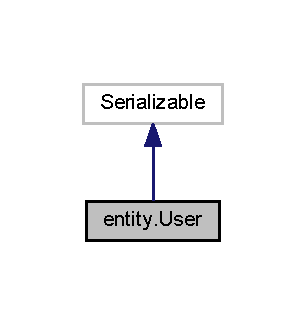
\includegraphics[width=147pt]{classentity_1_1_user__inherit__graph}
\end{center}
\end{figure}


Collaboration diagram for entity.\+User\+:\nopagebreak
\begin{figure}[H]
\begin{center}
\leavevmode
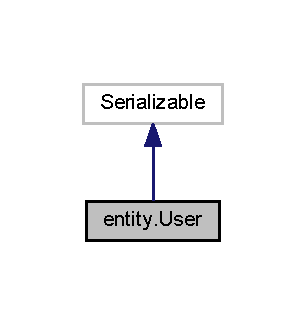
\includegraphics[width=147pt]{classentity_1_1_user__coll__graph}
\end{center}
\end{figure}
\subsection*{Public Member Functions}
\begin{DoxyCompactItemize}
\item 
\mbox{\Hypertarget{classentity_1_1_user_a930c504e6004ddb37035544fbd904166}\label{classentity_1_1_user_a930c504e6004ddb37035544fbd904166}} 
{\bfseries User} (String username, String password, String name, String surname, String mail)
\item 
\mbox{\Hypertarget{classentity_1_1_user_a030c1335a60b60d90e731b1438292d3b}\label{classentity_1_1_user_a030c1335a60b60d90e731b1438292d3b}} 
{\bfseries User} (\mbox{\hyperlink{classentity_1_1_usertype}{Usertype}} usertype, String username, String password, String name, String surname, String mail, Date born\+Dat)
\item 
\mbox{\Hypertarget{classentity_1_1_user_a4004338c97a54b7a80369b5aad8fad0f}\label{classentity_1_1_user_a4004338c97a54b7a80369b5aad8fad0f}} 
int {\bfseries get\+User\+Id} ()
\item 
\mbox{\Hypertarget{classentity_1_1_user_a58e8f4d8e357810b972d52dc1383013e}\label{classentity_1_1_user_a58e8f4d8e357810b972d52dc1383013e}} 
void {\bfseries set\+User\+Id} (int user\+Id)
\item 
\mbox{\Hypertarget{classentity_1_1_user_a050e73c7a9b10da8cec45c60afe9b942}\label{classentity_1_1_user_a050e73c7a9b10da8cec45c60afe9b942}} 
\mbox{\hyperlink{classentity_1_1_usertype}{Usertype}} {\bfseries get\+Usertype} ()
\item 
\mbox{\Hypertarget{classentity_1_1_user_a0981e69a22d9baed58f63d8e757ae7a7}\label{classentity_1_1_user_a0981e69a22d9baed58f63d8e757ae7a7}} 
void {\bfseries set\+Usertype} (\mbox{\hyperlink{classentity_1_1_usertype}{Usertype}} usertype)
\item 
\mbox{\Hypertarget{classentity_1_1_user_a346d96c8b90b4ba0446170f2bf913be8}\label{classentity_1_1_user_a346d96c8b90b4ba0446170f2bf913be8}} 
String {\bfseries get\+Username} ()
\item 
\mbox{\Hypertarget{classentity_1_1_user_a1b88018038c39d85b2e500f5134ca7c5}\label{classentity_1_1_user_a1b88018038c39d85b2e500f5134ca7c5}} 
void {\bfseries set\+Username} (String username)
\item 
\mbox{\Hypertarget{classentity_1_1_user_ac45f7a1da720c4bcc21ce365c29a74b4}\label{classentity_1_1_user_ac45f7a1da720c4bcc21ce365c29a74b4}} 
String {\bfseries get\+Password} ()
\item 
\mbox{\Hypertarget{classentity_1_1_user_a91eda90caa1220f6b2c0ec4aebbf6810}\label{classentity_1_1_user_a91eda90caa1220f6b2c0ec4aebbf6810}} 
void {\bfseries set\+Password} (String password)
\item 
\mbox{\Hypertarget{classentity_1_1_user_aadec9c3bcce34926a4e3dfe092499934}\label{classentity_1_1_user_aadec9c3bcce34926a4e3dfe092499934}} 
String {\bfseries get\+Name} ()
\item 
\mbox{\Hypertarget{classentity_1_1_user_afd002543b54320b13cb004b909083ce4}\label{classentity_1_1_user_afd002543b54320b13cb004b909083ce4}} 
void {\bfseries set\+Name} (String name)
\item 
\mbox{\Hypertarget{classentity_1_1_user_abc6c40b85eae27cc9ce6ff127767b47d}\label{classentity_1_1_user_abc6c40b85eae27cc9ce6ff127767b47d}} 
String {\bfseries get\+Surname} ()
\item 
\mbox{\Hypertarget{classentity_1_1_user_ad4d2d21374dd1352fe8d4d4349dbec0f}\label{classentity_1_1_user_ad4d2d21374dd1352fe8d4d4349dbec0f}} 
void {\bfseries set\+Surname} (String surname)
\item 
\mbox{\Hypertarget{classentity_1_1_user_ab5992e6dcc7b2cd7cf6a03b13b5ffa18}\label{classentity_1_1_user_ab5992e6dcc7b2cd7cf6a03b13b5ffa18}} 
String {\bfseries get\+Mail} ()
\item 
\mbox{\Hypertarget{classentity_1_1_user_a0b95b72010c13f08b795c04165ab4d5c}\label{classentity_1_1_user_a0b95b72010c13f08b795c04165ab4d5c}} 
void {\bfseries set\+Mail} (String mail)
\item 
\mbox{\Hypertarget{classentity_1_1_user_a6252395eaeb3df00686043ccabe886f4}\label{classentity_1_1_user_a6252395eaeb3df00686043ccabe886f4}} 
Date {\bfseries get\+Born\+Dat} ()
\item 
\mbox{\Hypertarget{classentity_1_1_user_af06d5955e7b981aba4858413817e422e}\label{classentity_1_1_user_af06d5955e7b981aba4858413817e422e}} 
void {\bfseries set\+Born\+Dat} (Date born\+Dat)
\item 
\mbox{\Hypertarget{classentity_1_1_user_a415c9d1d1003fb50953170650a8b369f}\label{classentity_1_1_user_a415c9d1d1003fb50953170650a8b369f}} 
String {\bfseries to\+String} ()
\end{DoxyCompactItemize}


\subsection{Detailed Description}
\mbox{\hyperlink{classentity_1_1_user}{User}} generated by hbm2java 

The documentation for this class was generated from the following file\+:\begin{DoxyCompactItemize}
\item 
src/main/java/entity/User.\+java\end{DoxyCompactItemize}

\hypertarget{classentity_1_1_usertype}{}\section{entity.\+Usertype Class Reference}
\label{classentity_1_1_usertype}\index{entity.\+Usertype@{entity.\+Usertype}}


Inheritance diagram for entity.\+Usertype\+:\nopagebreak
\begin{figure}[H]
\begin{center}
\leavevmode
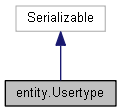
\includegraphics[width=163pt]{classentity_1_1_usertype__inherit__graph}
\end{center}
\end{figure}


Collaboration diagram for entity.\+Usertype\+:\nopagebreak
\begin{figure}[H]
\begin{center}
\leavevmode
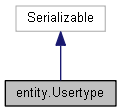
\includegraphics[width=163pt]{classentity_1_1_usertype__coll__graph}
\end{center}
\end{figure}
\subsection*{Public Member Functions}
\begin{DoxyCompactItemize}
\item 
\mbox{\Hypertarget{classentity_1_1_usertype_a3f17f72e004920b8d0099586a5b016fe}\label{classentity_1_1_usertype_a3f17f72e004920b8d0099586a5b016fe}} 
{\bfseries Usertype} (String usertype)
\item 
\mbox{\Hypertarget{classentity_1_1_usertype_aa9776ce9c7de7443a232c0531d78ea8b}\label{classentity_1_1_usertype_aa9776ce9c7de7443a232c0531d78ea8b}} 
{\bfseries Usertype} (String usertype, String description)
\item 
\mbox{\Hypertarget{classentity_1_1_usertype_a361cfd2f23d71f1ec7e69aa55e5f013c}\label{classentity_1_1_usertype_a361cfd2f23d71f1ec7e69aa55e5f013c}} 
int {\bfseries get\+Usertype\+Id} ()
\item 
\mbox{\Hypertarget{classentity_1_1_usertype_ad05f418dbd08027c7afac5e4af7d2254}\label{classentity_1_1_usertype_ad05f418dbd08027c7afac5e4af7d2254}} 
void {\bfseries set\+Usertype\+Id} (int usertype\+Id)
\item 
\mbox{\Hypertarget{classentity_1_1_usertype_ad300a2783e57d8690d9db0c3b464737b}\label{classentity_1_1_usertype_ad300a2783e57d8690d9db0c3b464737b}} 
String {\bfseries get\+Usertype} ()
\item 
\mbox{\Hypertarget{classentity_1_1_usertype_ac4220b848c369fd726b0c8bebc8dbcf3}\label{classentity_1_1_usertype_ac4220b848c369fd726b0c8bebc8dbcf3}} 
void {\bfseries set\+Usertype} (String usertype)
\item 
\mbox{\Hypertarget{classentity_1_1_usertype_a1699b78e303deb9b70224bf863b08063}\label{classentity_1_1_usertype_a1699b78e303deb9b70224bf863b08063}} 
String {\bfseries get\+Description} ()
\item 
\mbox{\Hypertarget{classentity_1_1_usertype_ab274da7bcfaa15606599fc856b958d24}\label{classentity_1_1_usertype_ab274da7bcfaa15606599fc856b958d24}} 
void {\bfseries set\+Description} (String description)
\item 
\mbox{\Hypertarget{classentity_1_1_usertype_a4211735d5a357a4dbd778c1b1aa4b7e0}\label{classentity_1_1_usertype_a4211735d5a357a4dbd778c1b1aa4b7e0}} 
String {\bfseries to\+String} ()
\end{DoxyCompactItemize}


\subsection{Detailed Description}
\mbox{\hyperlink{classentity_1_1_usertype}{Usertype}} generated by hbm2java 

The documentation for this class was generated from the following file\+:\begin{DoxyCompactItemize}
\item 
src/main/java/entity/Usertype.\+java\end{DoxyCompactItemize}

\hypertarget{classentity_1_1_workstation}{}\section{entity.\+Workstation Class Reference}
\label{classentity_1_1_workstation}\index{entity.\+Workstation@{entity.\+Workstation}}


Inheritance diagram for entity.\+Workstation\+:
% FIG 0


Collaboration diagram for entity.\+Workstation\+:
% FIG 1
\subsection*{Public Member Functions}
\begin{DoxyCompactItemize}
\item 
\mbox{\Hypertarget{classentity_1_1_workstation_a377e0a2bbe7044cc7f486bae0ea8ed67}\label{classentity_1_1_workstation_a377e0a2bbe7044cc7f486bae0ea8ed67}} 
{\bfseries Workstation} (String workstation\+Nam)
\item 
\mbox{\Hypertarget{classentity_1_1_workstation_a22288e3495ba499b6bde23eb07f7101b}\label{classentity_1_1_workstation_a22288e3495ba499b6bde23eb07f7101b}} 
{\bfseries Workstation} (\mbox{\hyperlink{classentity_1_1_segment}{Segment}} segment, String workstation\+Nam, String description, Boolean state, Set carrieses\+For\+Destiny\+Workstation\+Id, Set carrieses\+For\+Initial\+Workstation\+Id)
\item 
\mbox{\Hypertarget{classentity_1_1_workstation_abb73425f42c9c651fdd58e06e9dd5e8b}\label{classentity_1_1_workstation_abb73425f42c9c651fdd58e06e9dd5e8b}} 
int {\bfseries get\+Workstation\+Id} ()
\item 
\mbox{\Hypertarget{classentity_1_1_workstation_a34dbc056f3a0bfa3a94aebfc8a0f0d68}\label{classentity_1_1_workstation_a34dbc056f3a0bfa3a94aebfc8a0f0d68}} 
void {\bfseries set\+Workstation\+Id} (int workstation\+Id)
\item 
\mbox{\Hypertarget{classentity_1_1_workstation_a41f03757564ca8adcdc0a062c33f99d4}\label{classentity_1_1_workstation_a41f03757564ca8adcdc0a062c33f99d4}} 
\mbox{\hyperlink{classentity_1_1_segment}{Segment}} {\bfseries get\+Segment} ()
\item 
\mbox{\Hypertarget{classentity_1_1_workstation_a419f3d517914ff99b9c3b1a151deaf37}\label{classentity_1_1_workstation_a419f3d517914ff99b9c3b1a151deaf37}} 
void {\bfseries set\+Segment} (\mbox{\hyperlink{classentity_1_1_segment}{Segment}} segment)
\item 
\mbox{\Hypertarget{classentity_1_1_workstation_a8af3245910985e27ce7e8d5d1acd3e2d}\label{classentity_1_1_workstation_a8af3245910985e27ce7e8d5d1acd3e2d}} 
String {\bfseries get\+Workstation\+Nam} ()
\item 
\mbox{\Hypertarget{classentity_1_1_workstation_ae21df43c124cfd95deb4845726473b19}\label{classentity_1_1_workstation_ae21df43c124cfd95deb4845726473b19}} 
void {\bfseries set\+Workstation\+Nam} (String workstation\+Nam)
\item 
\mbox{\Hypertarget{classentity_1_1_workstation_ae79cd9019eb03d8526727c98ade26905}\label{classentity_1_1_workstation_ae79cd9019eb03d8526727c98ade26905}} 
String {\bfseries get\+Description} ()
\item 
\mbox{\Hypertarget{classentity_1_1_workstation_ad164f196f2a925758dac0e9b9e28484b}\label{classentity_1_1_workstation_ad164f196f2a925758dac0e9b9e28484b}} 
void {\bfseries set\+Description} (String description)
\item 
\mbox{\Hypertarget{classentity_1_1_workstation_a49be3c2bef3d42a5596844c603712061}\label{classentity_1_1_workstation_a49be3c2bef3d42a5596844c603712061}} 
Boolean {\bfseries get\+State} ()
\item 
\mbox{\Hypertarget{classentity_1_1_workstation_a33d712bc34bd23dcf56492d3dd562635}\label{classentity_1_1_workstation_a33d712bc34bd23dcf56492d3dd562635}} 
void {\bfseries set\+State} (Boolean state)
\item 
\mbox{\Hypertarget{classentity_1_1_workstation_a0da8d108a3195e74a9cd37a48ac80e0d}\label{classentity_1_1_workstation_a0da8d108a3195e74a9cd37a48ac80e0d}} 
Set {\bfseries get\+Carrieses\+For\+Destiny\+Workstation\+Id} ()
\item 
\mbox{\Hypertarget{classentity_1_1_workstation_a9d7abfff67413a398a7927928caa8f35}\label{classentity_1_1_workstation_a9d7abfff67413a398a7927928caa8f35}} 
void {\bfseries set\+Carrieses\+For\+Destiny\+Workstation\+Id} (Set carrieses\+For\+Destiny\+Workstation\+Id)
\item 
\mbox{\Hypertarget{classentity_1_1_workstation_a9cc802a3b25ea2b483b776ccd0f4a24a}\label{classentity_1_1_workstation_a9cc802a3b25ea2b483b776ccd0f4a24a}} 
Set {\bfseries get\+Carrieses\+For\+Initial\+Workstation\+Id} ()
\item 
\mbox{\Hypertarget{classentity_1_1_workstation_a5ac57917431af5a9a85ada5a74f7c64e}\label{classentity_1_1_workstation_a5ac57917431af5a9a85ada5a74f7c64e}} 
void {\bfseries set\+Carrieses\+For\+Initial\+Workstation\+Id} (Set carrieses\+For\+Initial\+Workstation\+Id)
\end{DoxyCompactItemize}


\subsection{Detailed Description}
\mbox{\hyperlink{classentity_1_1_workstation}{Workstation}} generated by hbm2java 

The documentation for this class was generated from the following file\+:\begin{DoxyCompactItemize}
\item 
D\+:/\+Users/user/\+Documents/\+M\+O\+N\+D\+R\+A/3.\+M\+A\+I\+L\+A/\+P\+O\+P\+B\+L5/\+G\+I\+T/e\+Jkiva\+\_\+\+P\+O\+P\+B\+L5/e\+Jkiva/src/main/java/entity/Workstation.\+java\end{DoxyCompactItemize}

%--- End generated contents ---

% Index
\backmatter
\newpage
\phantomsection
\clearemptydoublepage
\addcontentsline{toc}{chapter}{Index}
\printindex

\end{document}
